\newpage
\subsection*{Komponenten}
\label{sec:Kaeltetechnik}


Da sich diese Masterarbeit mit dem Aufbau eines Prüfstandes zur Untersuchung von Abtaumethoden einer Kompressionskälteanlage beschäftigt, wird in den folgenden Kapiteln ausschließlich auf diese Technologie eingegangen. Die Kälteanlage entzieht über einen Luftkühler der Umgebung Wärme. Die Wärmeübertragung findet unter erzwungener Konvektion statt, da der Luftkühler mit einem Ventilator ausgestattet ist. Für weitere Informationen bezüglich der anderen Technologien sei an dieser Stelle auf die Literatur \citep{Baehr2013} and \citep{Grote2014} verwiesen.

Die Komponenten für einen einfachen Kaltdampfprozess  sind folgende vier Komponenten:

\begin{itemize}
\item der Kompressor
\item der Verflüssiger 
\item das Expansionsventil
\item der Verdampfer. 
\end{itemize}

In Abbildung \ref{fig:einfacher Kältekreislauf} sind die vier Komponenten mit ihren Zustandspunkten dargestellt.

\begin{figure}[htb]
\centering		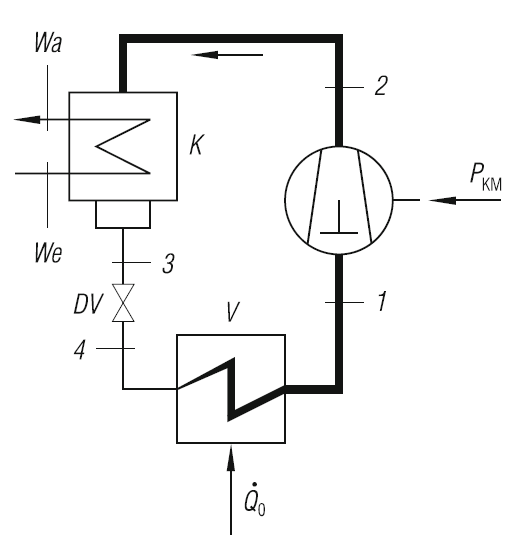
\includegraphics[width=0.50\textwidth]{Pictures/Kaltekreislauf_beahr.png}
\caption{Einfacher Kältekreislauf \citep{Baehr2013}}
\label{fig:einfacher Kältekreislauf}
\end{figure}

\subsubsection*{Der Kompressor}
Der Kompressor bildet das Herzstück der Kälteanlage. Er verdichtet das gasförmige Kältemittel von niedrigem Druck auf ein höheres Druckniveau. Um diese Arbeit zu verrichten, wird der Kompressor mit elektrischer Energie versorgt. %Den Kompressor gibt es in verschiedenen Bauvarianten. Die zwei wichtigsten Bauvarianten sind der \textit{Hubkolben-} und der \textit{Rotationskolbenverdichter}. Kompressoren zwischen offenen, halbhermetischen und vollhermetischen Ausführungen unterschieden. Schrauben-, Scroll- sowie Turboverdichter sind Bauarten der \textit{Rotationskolbenverdichter}. 

\subsubsection*{Der Verflüssiger}

Dem Kältemittel wird im Verflüssiger auf einem hohen Druckniveau Wärme entzogen. Der Verflüssiger entzieht dem überhitzten gasförmigen Kältemittel Wärme. Beim Austritt aus dem Verflüssiger ist das Kältemittel meist vollständig flüssig. 
%Um einen Wärmeentzug zu bewerkstelligen, gibt es drei Bautypen:

%\begin{itemize}
%\item Wassergekühlte Verflüssiger
%\item Luftgekühlte Verflüssiger
%\item Verdunstungsverflüsssiger
%\end{itemize}

Verflüssiger unterscheiden sich hinsichtlich des Wärmeabführenden Mediums durch Bauform, Baugrösse und Hilfsenergien.

%Wassergekühlte Verflüssiger können, aufgrund der besseren Wärmeübertragung verglichen mit Luftkühlern, sehr kompakt gebaut werden. Eine typische Bauform ist der \textit{Bündelrohrverflüssiger}.
%In der Praxis werden am häufigsten luftgekühlte Verflüssiger eingesetzt. Um die gleiche Kühlleistung wie bei einem wassergekühlter Verflüssiger zu erreichen, werden Lamellen und Ventilatoren eingesetzt. Die Lamellen vergrößern die Fläche für die Wärmeübertragung mit der Luft. Ventilatoren ermöglichen durch einen höheren Luftdurchsatz und der daraus resultierendem höheren Wärmeübertragung eine größere Kühlleistung und eine kompaktere Bauform der Wärmeübertragers. Diese Variante hat den Vorteil, dass sie einen wartungsfreien Betrieb  sowie eine einfache Reinigung ermöglicht.


\subsubsection*{Das Expansionsventil}

Das Expansionsventil ist ein Überhitzungsregler und regelt das in den Verdampfer eingespritzen Kältmittelmassenstrom. Die Zuführung des Kältemittels erfolgt über eine Druckdifferenz. Durch eine lokale Verengung des Strömungquerschnitts verringet sich der Druck des durchfließenden Kältemittels. Das Kältemittel vergrößert sein Volumen und es kommt zur Expansion. Im idealen Fall wird bei diesem Prozess auch keine Wärme abgeführt; der Prozess ist \textit{isenthalp}. 
%Das Expansionsventil trennt zusammen mit dem Kompressor die zwei Druckseiten des Kältekreislaufes.
 Es gibt bei Expansionsventile sowohl  regelbare als auch nicht regelbare Ausführungen.  Geregelte Expansionsventile werden in mittleren und großen Kälteanlagen eingesetzt. Die Regelung erfolgt durch die Querschnittsänderung und dem damit einhergehendem Druckabfall.  

\subsubsection*{Der Verdampfer}

Das Kältemittel wird in den Verdampfer eingespritzt. Das Kältemittel verdampft und entzieht seiner Umgebung dabei Wärme. Aufgrund der vielfältigen Anforderungen an Verdampfer, gibt es eine Vielzahl an Bauarten für Verdampfer.

Um eine möglichst große spezifische Kälteleistung zu ermöglichen, werden wie beim Verflüssiger auch Ventilatoren eingesetzt. Die Ventilatoren erzwingen einen Luftstrom durch den Verdampfer und erhöhen damit die Wärmeübertragung zwischen der Luft und den Verdampferrohren. Es wird von \textit{erzwungener Konvektion} gesprochen. 

